\documentclass[12pt, a4paper]{article}

% --- Paquetes básicos ---
\usepackage[utf8]{inputenc}
\usepackage[spanish]{babel}
\usepackage[margin=2.5cm]{geometry}
\usepackage{graphicx}
\usepackage{float}
\usepackage{amsmath, amssymb}
\usepackage{fancyhdr}

% --- Configuración del Título ---
\title{Bloque 2: Simulación de Carga de Trabajo y Monitorización}
\author{Juan Reche Aguilar}
\date{\today}

% --- Configuración de Encabezados ---
\pagestyle{fancy}
\fancyhf{}
\rhead{Ingeniería de Servidores}
\lhead{Juan Reche Aguilar}
\cfoot{\thepage}

\begin{document}

\maketitle

\tableofcontents
\newpage

\section{ Ejercicio 4.4.1. Monitorización con Grafana + Prometheus.. }

\subsection{Guía con capturas.}

\begin{figure}[H]
    \centering

    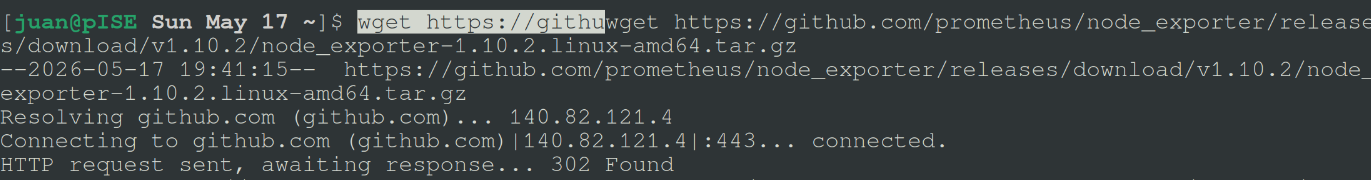
\includegraphics[width=1\textwidth]{../../capturas4/seccion4/1get_prometeus.png}

    \caption{Descarga de Prometheus.}

\end{figure}

\begin{figure}[H]
    \centering

    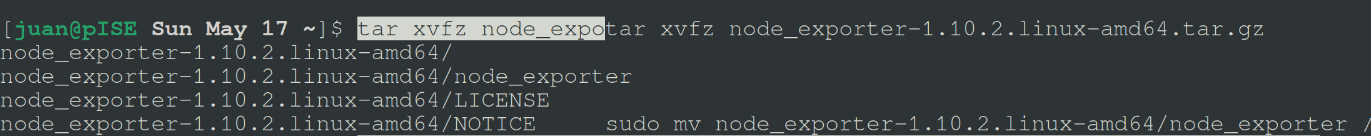
\includegraphics[width=1\textwidth]{../../capturas4/seccion4/2tar_exporter.png}

    \caption{Descompresión del Exporter.}

\end{figure}

\begin{figure}[H]
    \centering

    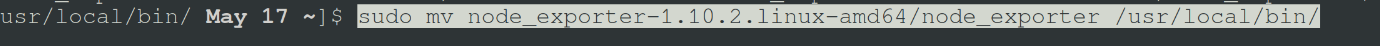
\includegraphics[width=1\textwidth]{../../capturas4/seccion4/3mover_exporter.png}

    \caption{Movemos el programa a la carpeta de archivos binarios.}

\end{figure}

\begin{figure}[H]
    \centering

    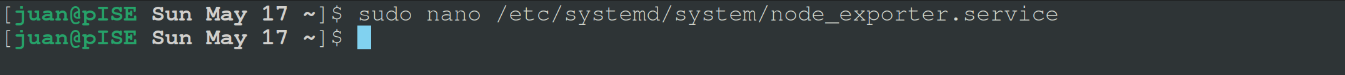
\includegraphics[width=1\textwidth]{../../capturas4/seccion4/4conf_exporter_1.png}

    \caption{Archivo de configuración del sistema para node\_exporter.}

\end{figure}

\begin{figure}[H]
    \centering

    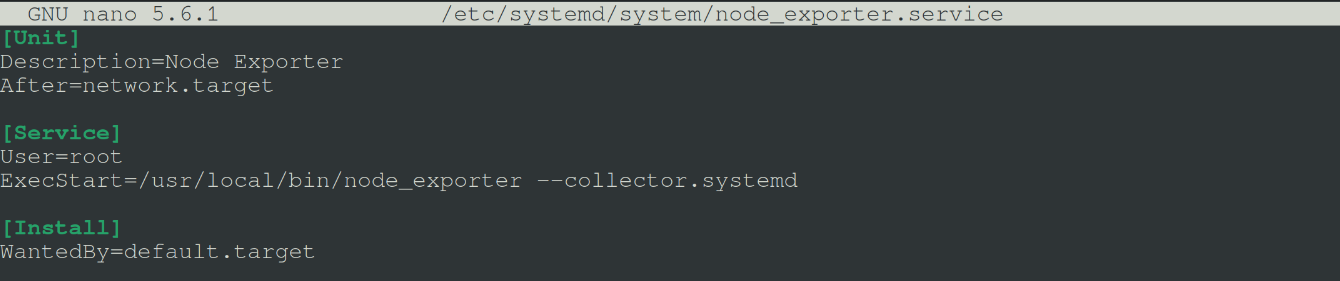
\includegraphics[width=1\textwidth]{../../capturas4/seccion4/5conf_exporter_2.png}

    \caption{Configuración del node\_exporter.}

\end{figure}

La intención de esta configuración es que el programa se ejecute automáticamente al iniciar el sistema, 
indicándole que se ejecute después de la interfaz de red, así como la carpeta donde se encuentra y sus permisos.

\begin{figure}[H]
    \centering

    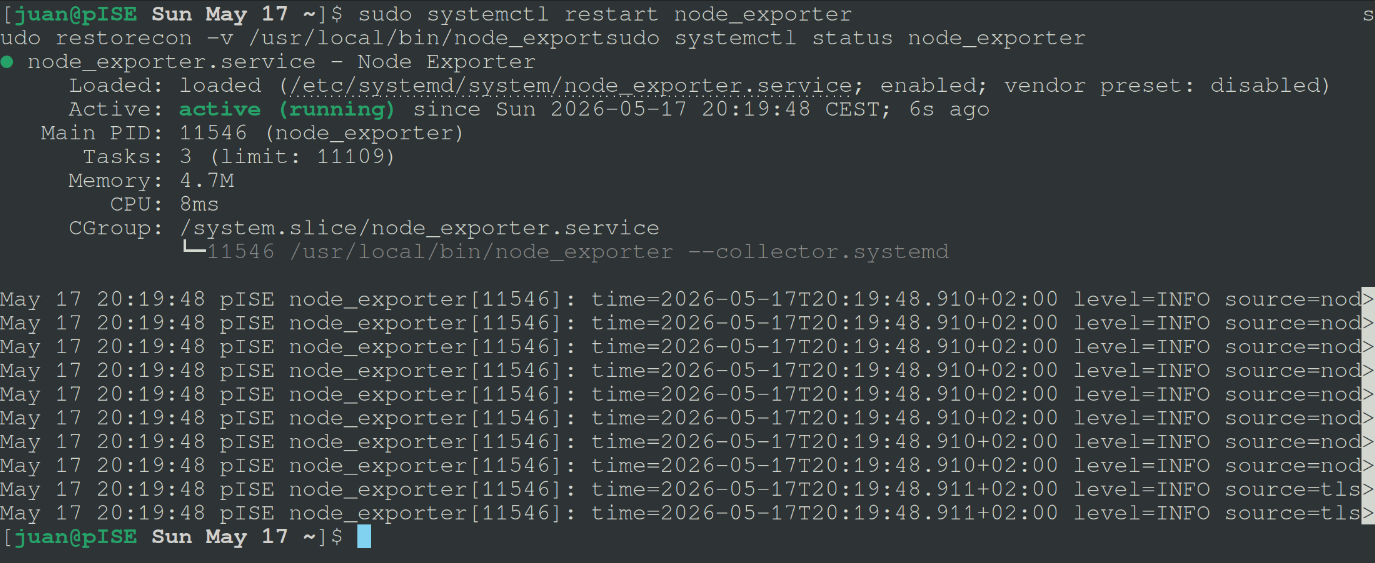
\includegraphics[width=1\textwidth]{../../capturas4/seccion4/6encender_exporter.png}

    \caption{Encendido y status de node\_exporter.}

\end{figure}

Realmente es un reinicio debido a que ya se intento iniciarlo pero dio error debido a la red, para solucionarlo 
se ejecuto anteriormente:
\begin{verbatim}
sudo firewall-cmd --add-port=9100/tcp --permanent
sudo firewall-cmd --reload
\end{verbatim}

\begin{figure}[H]
    \centering

    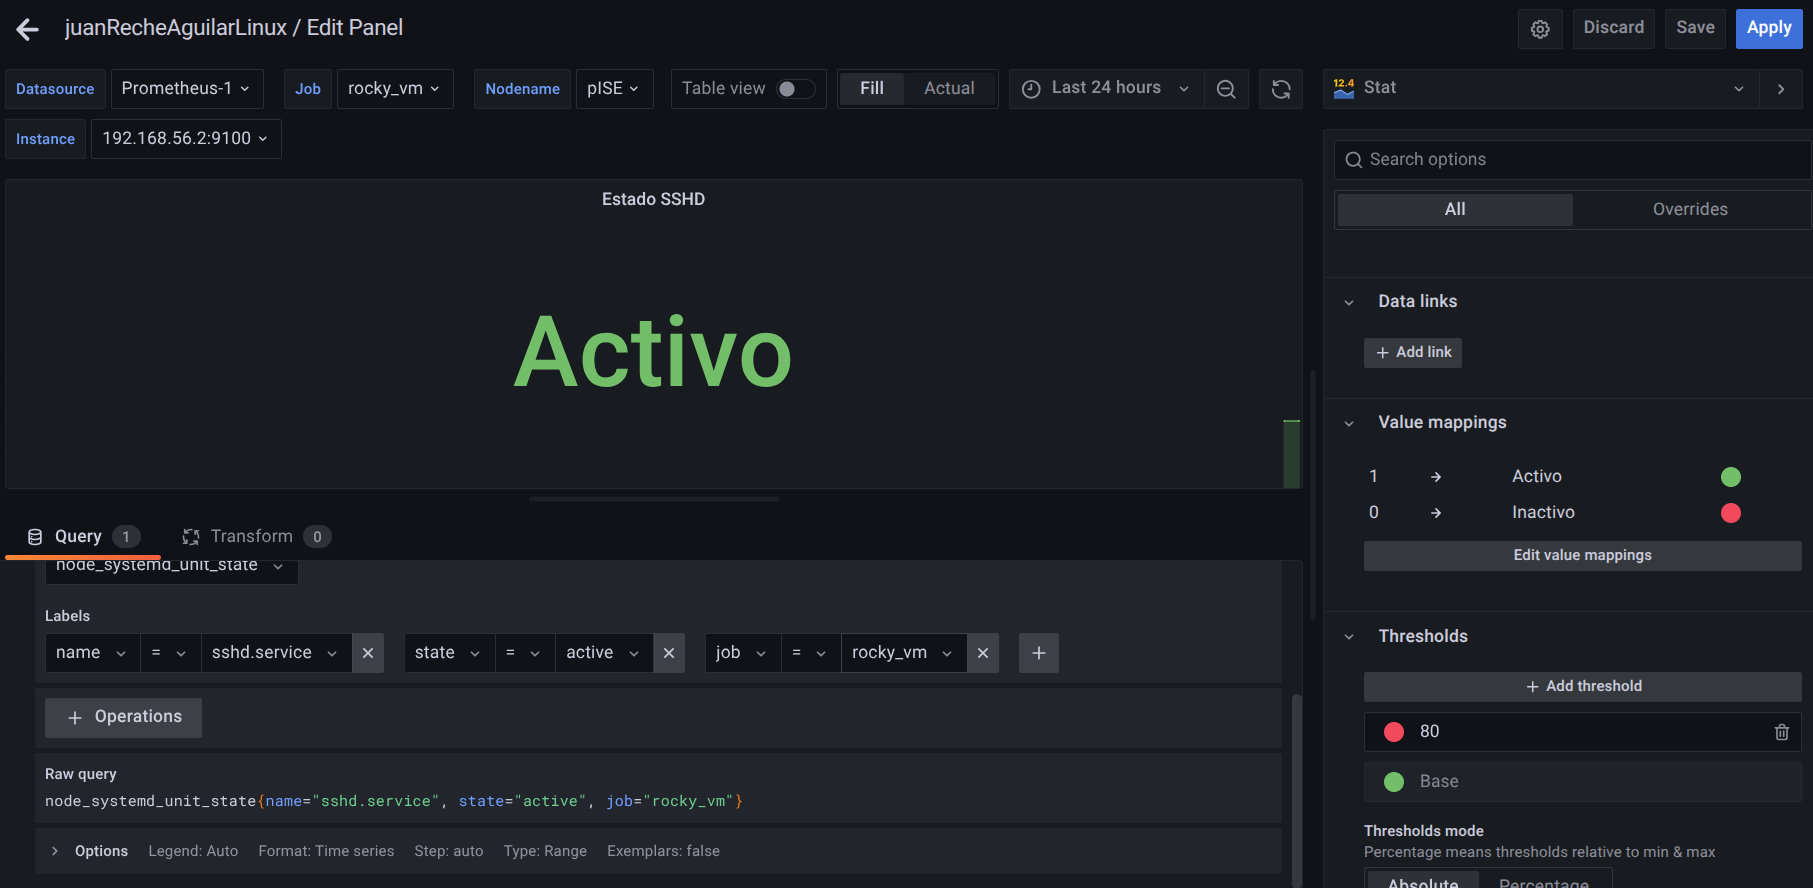
\includegraphics[width=1\textwidth]{../../capturas4/seccion4/7edit_panel_ssh.png}

    \caption{Creación del panel para monitorizar el puerto SSH (funcionamiento idéntico al de apache).}

\end{figure}

\begin{figure}[H]
    \centering

    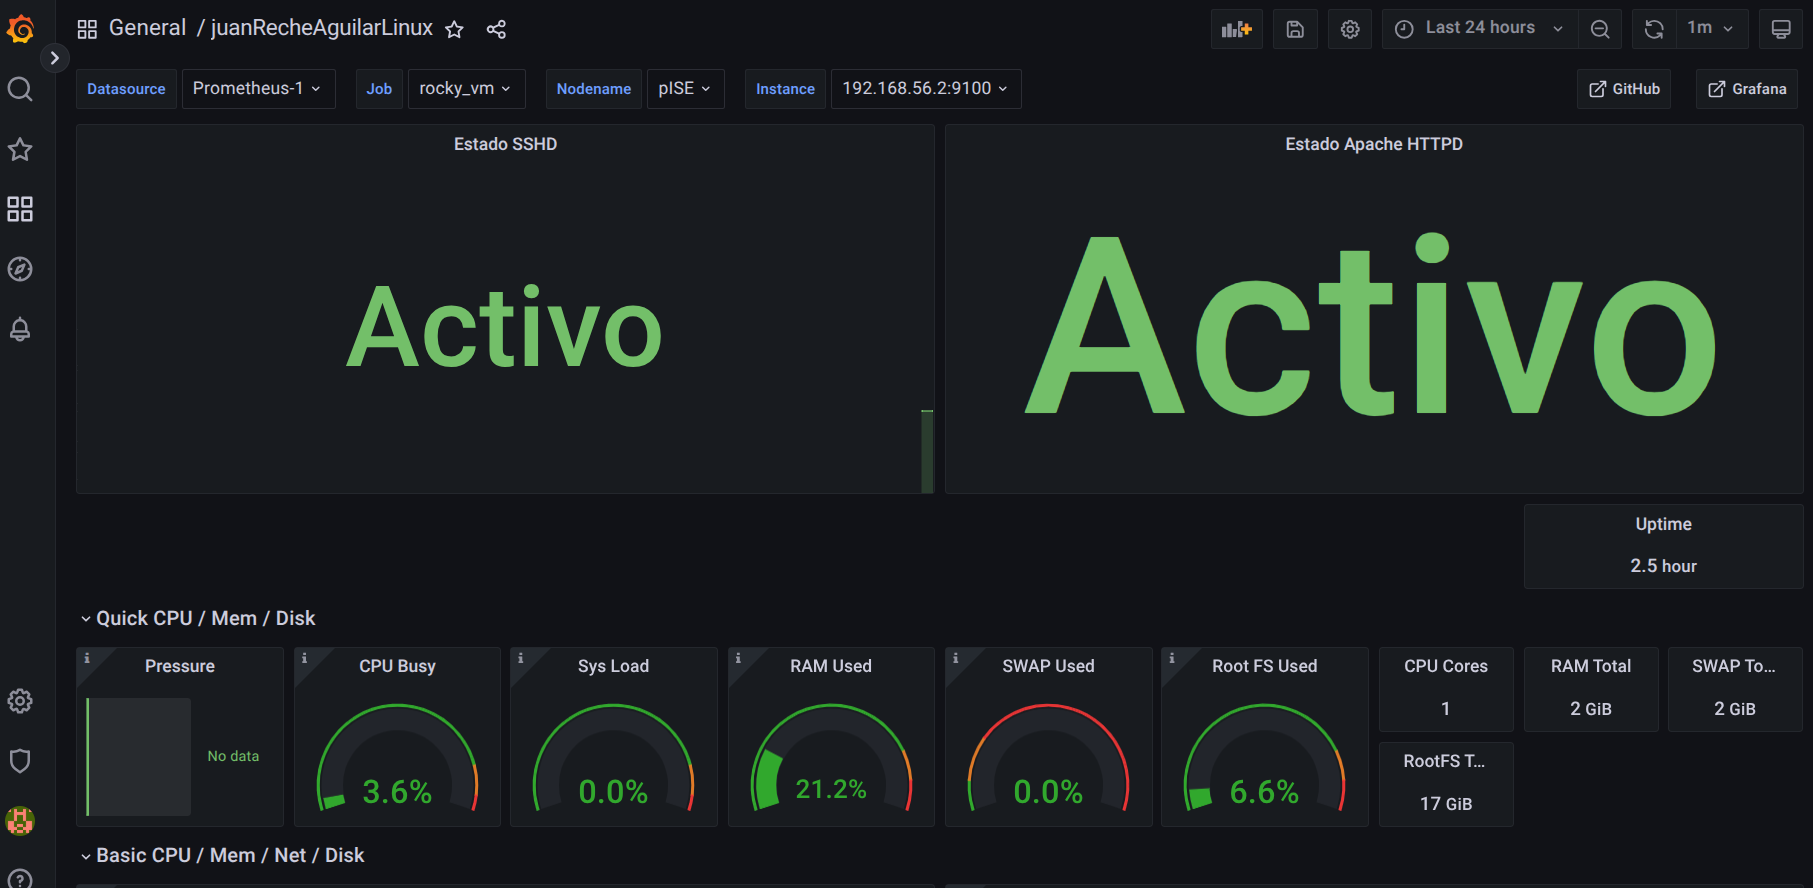
\includegraphics[width=1\textwidth]{../../capturas4/seccion4/8ssh_http_activo.png}

    \caption{Ambos puertos activos.}

\end{figure}

\begin{figure}[H]
    \centering

    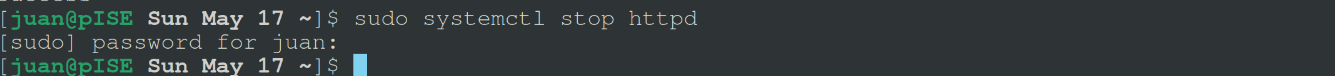
\includegraphics[width=1\textwidth]{../../capturas4/seccion4/9stop_http.png}

    \caption{Detención del servicio HTTP.}

\end{figure}

\begin{figure}[H]
    \centering

    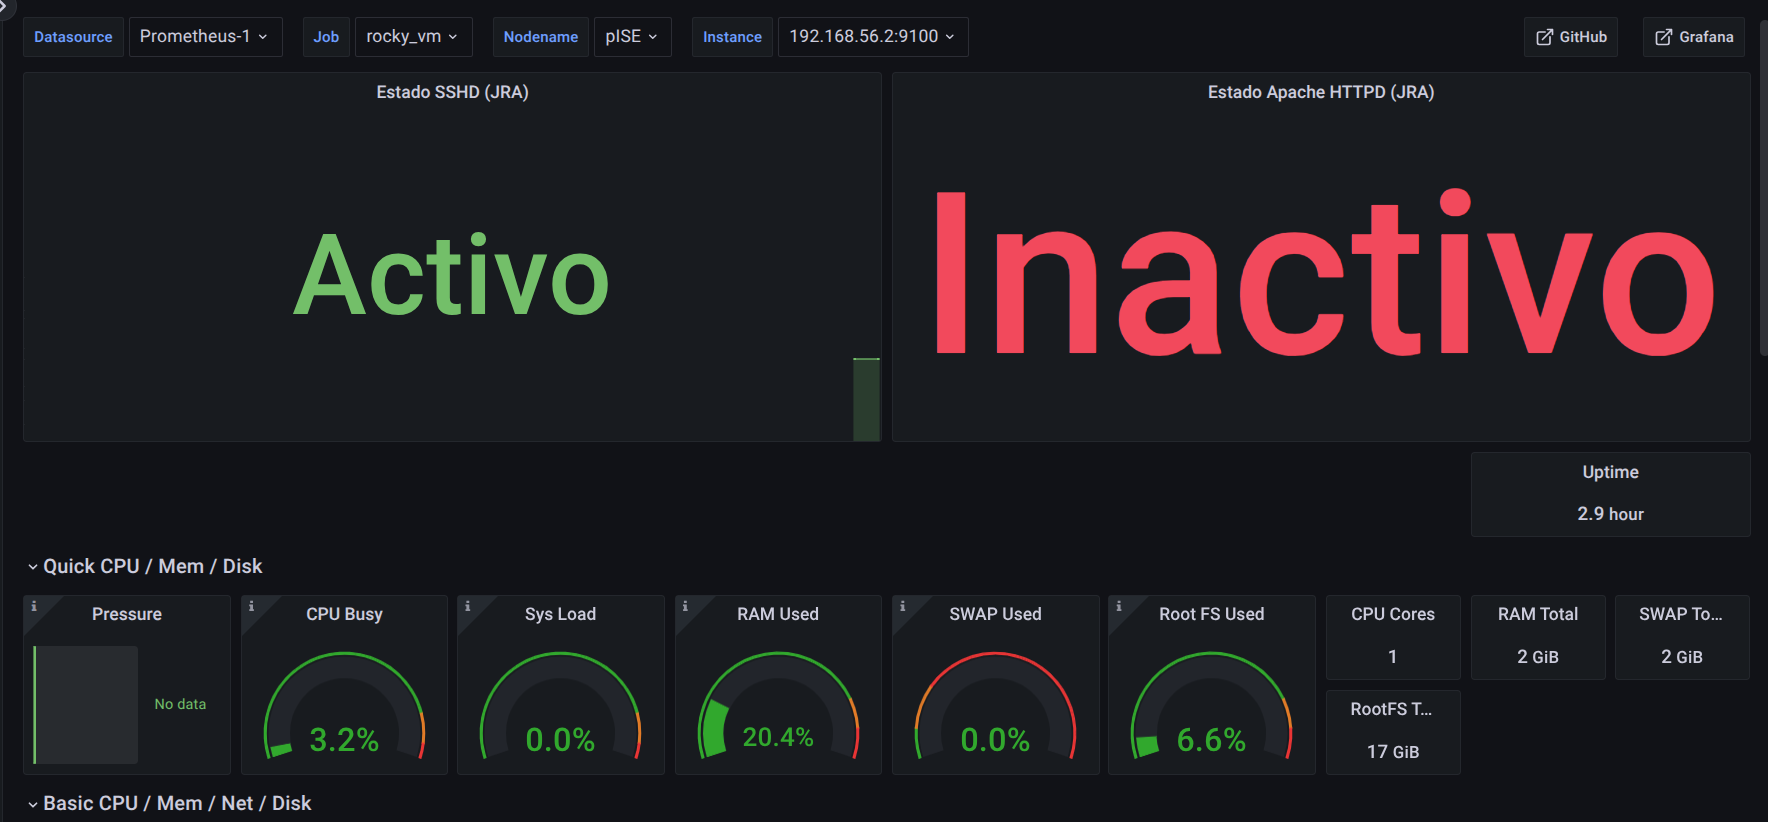
\includegraphics[width=1\textwidth]{../../capturas4/seccion4/10ssh_si_http_no.png}

    \caption{Puerto SSH activo y puerto HTTP detenido.}

\end{figure}

Podemos ver como en un principio ambos puertos estaban activos, 
pero al detener el servicio HTTP, el puerto 80 se detuvo y el panel de Grafana lo reflejó.

\begin{figure}[H]
    \centering

    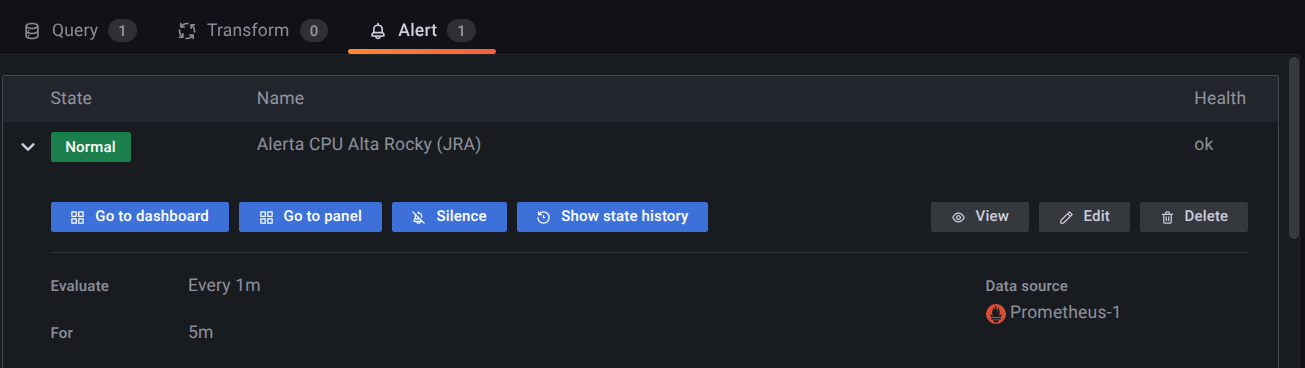
\includegraphics[width=1\textwidth]{../../capturas4/seccion4/11alerta.png}

    \caption{Alerta creada para el rendimiento del cpu (estado normal).}

\end{figure}

\begin{figure}[H]
    \centering

    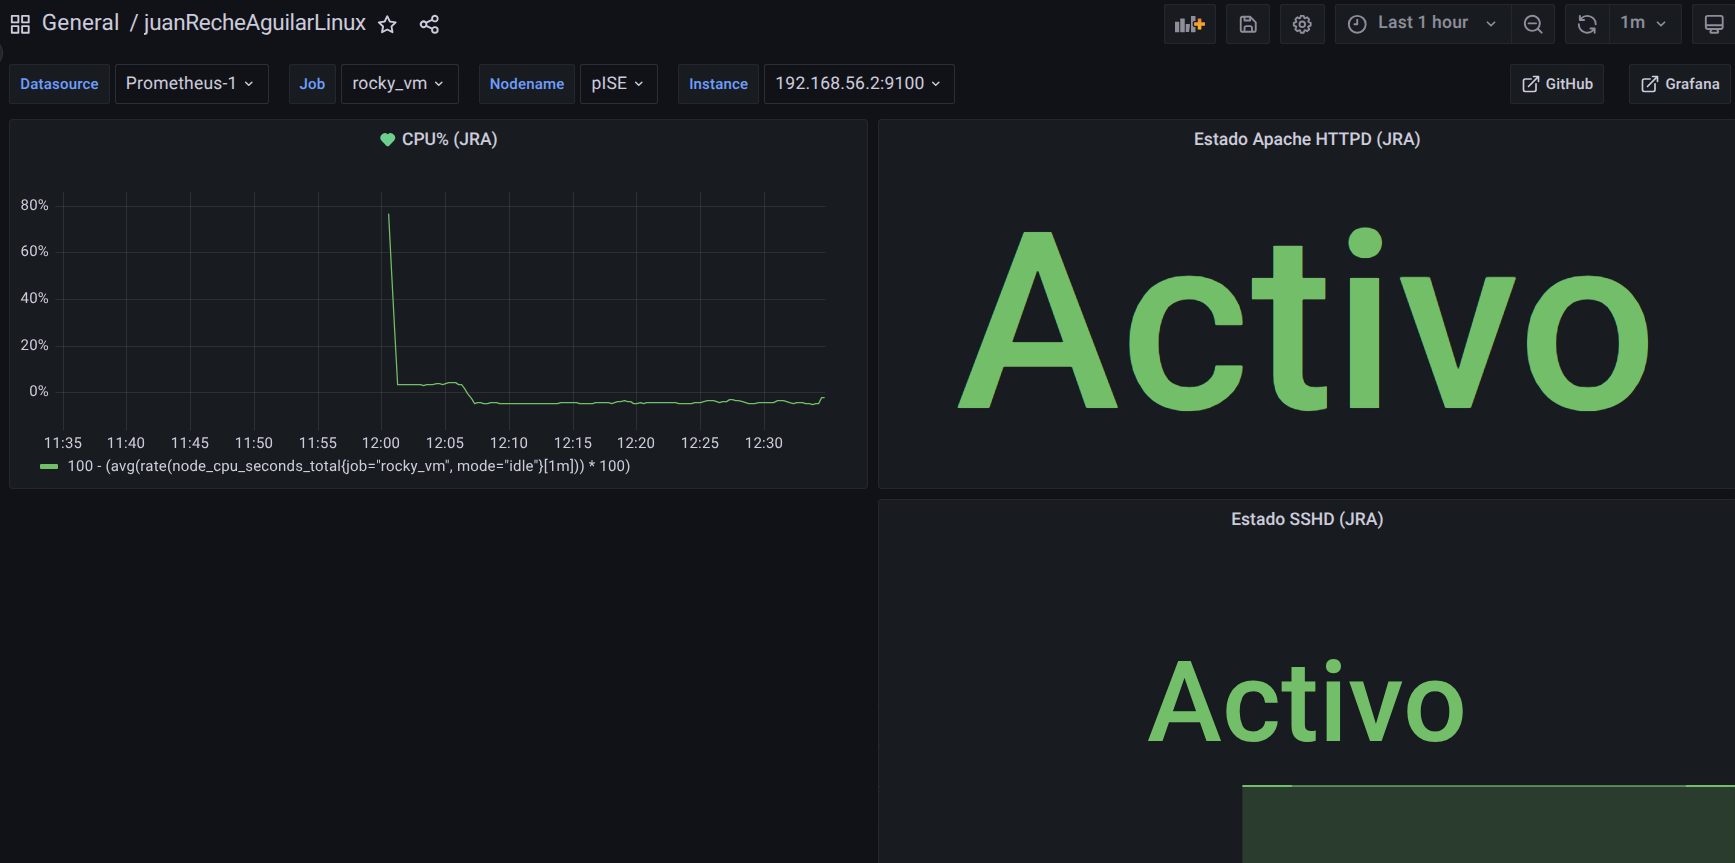
\includegraphics[width=1\textwidth]{../../capturas4/seccion4/12estado_reposo.png}

    \caption{Estado de reposo del sistema antes de ejecutar stress. 
    (esta captura se ha realizado después de realizar la practica para mostrar el consumo de CPU en reposo).}

\end{figure}

\begin{figure}[H]
    \centering

    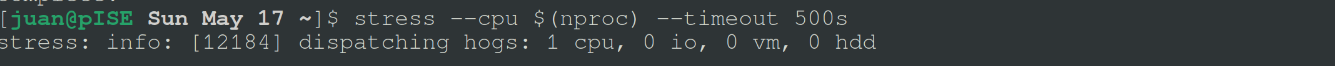
\includegraphics[width=1\textwidth]{../../capturas4/seccion4/13stress.png}

    \caption{Ejecución del comando stress.}

\end{figure}

\begin{figure}[H]
    \centering

    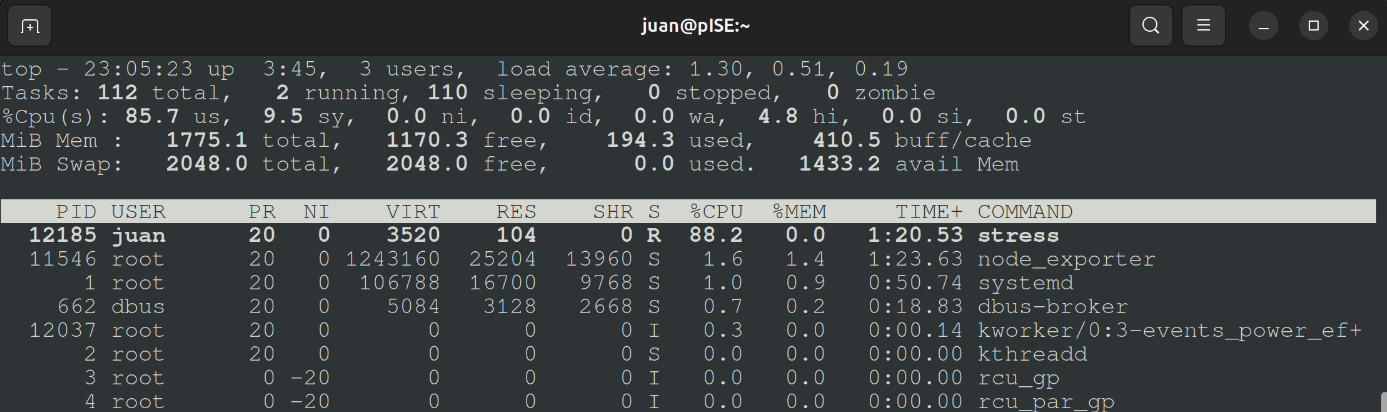
\includegraphics[width=1\textwidth]{../../capturas4/seccion4/14top_stress_funciona.png}

    \caption{Verificamos que el comando stress funciona correctamente y está consumiendo recursos.}

\end{figure}

\begin{figure}[H]
    \centering

    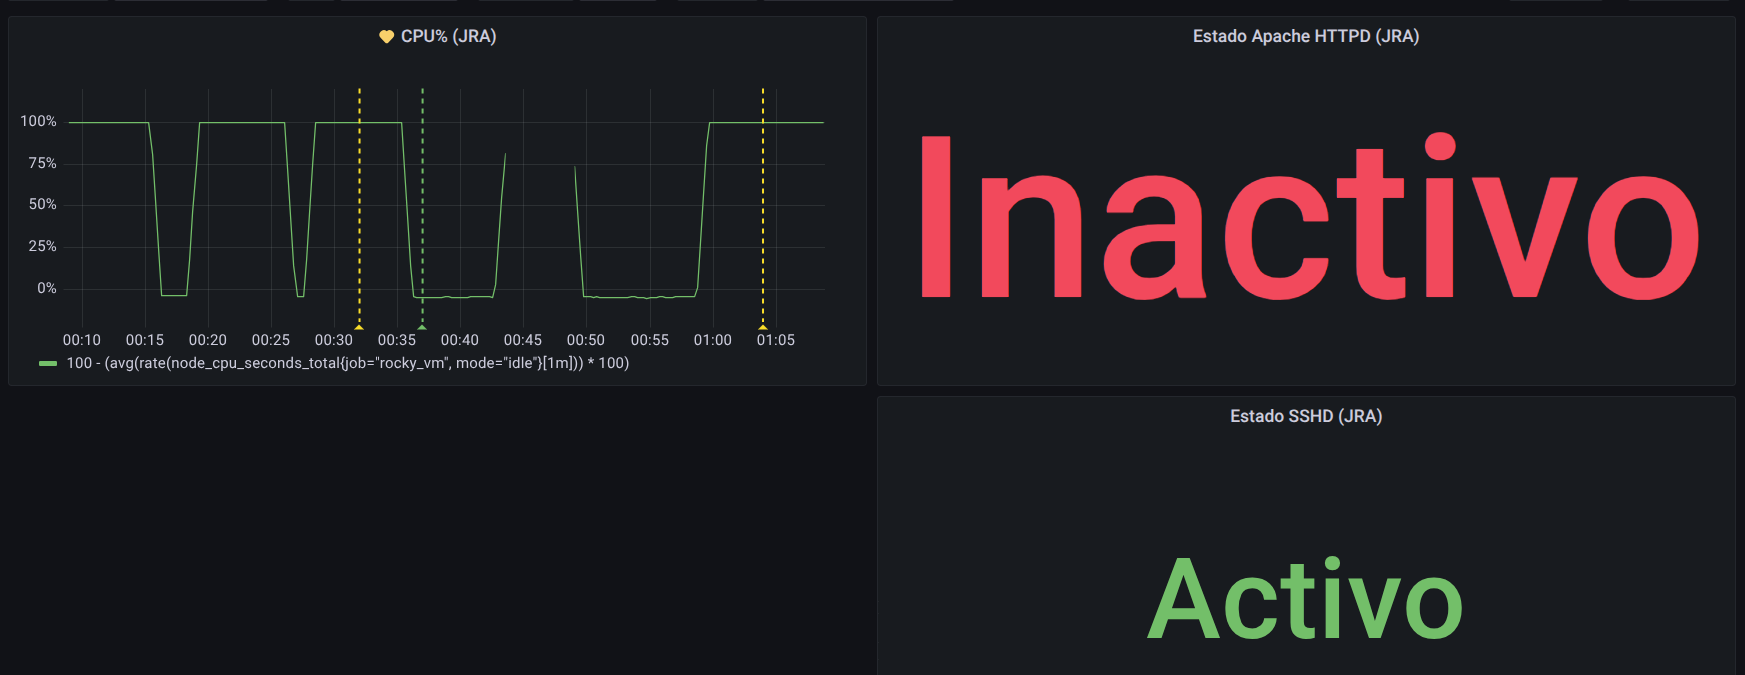
\includegraphics[width=1\textwidth]{../../capturas4/seccion4/15proxima_alerta.png}

    \caption{Acercándonos a la alerta.}

\end{figure}

Podemos ver como el consumo de CPU se ha disparado a causa del comando stress, 
y estamos a punto de alcanzar el umbral de la alerta que hemos creado. 

\begin{figure}[H]
    \centering

    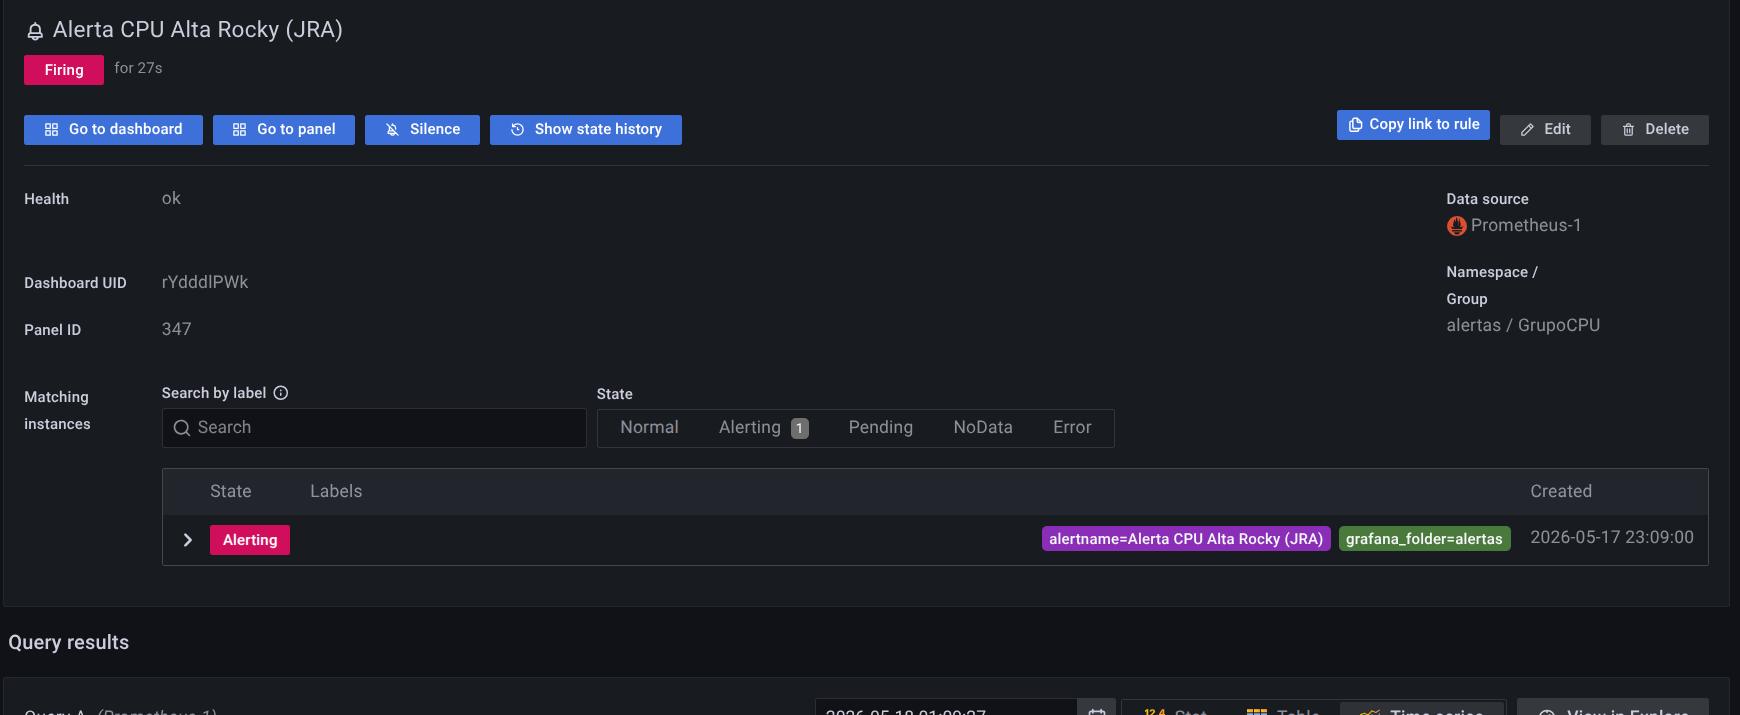
\includegraphics[width=1\textwidth]{../../capturas4/seccion4/16alerta_alertando.png}

    \caption{Alerta activada.}

\end{figure}

\begin{figure}[H]
    \centering

    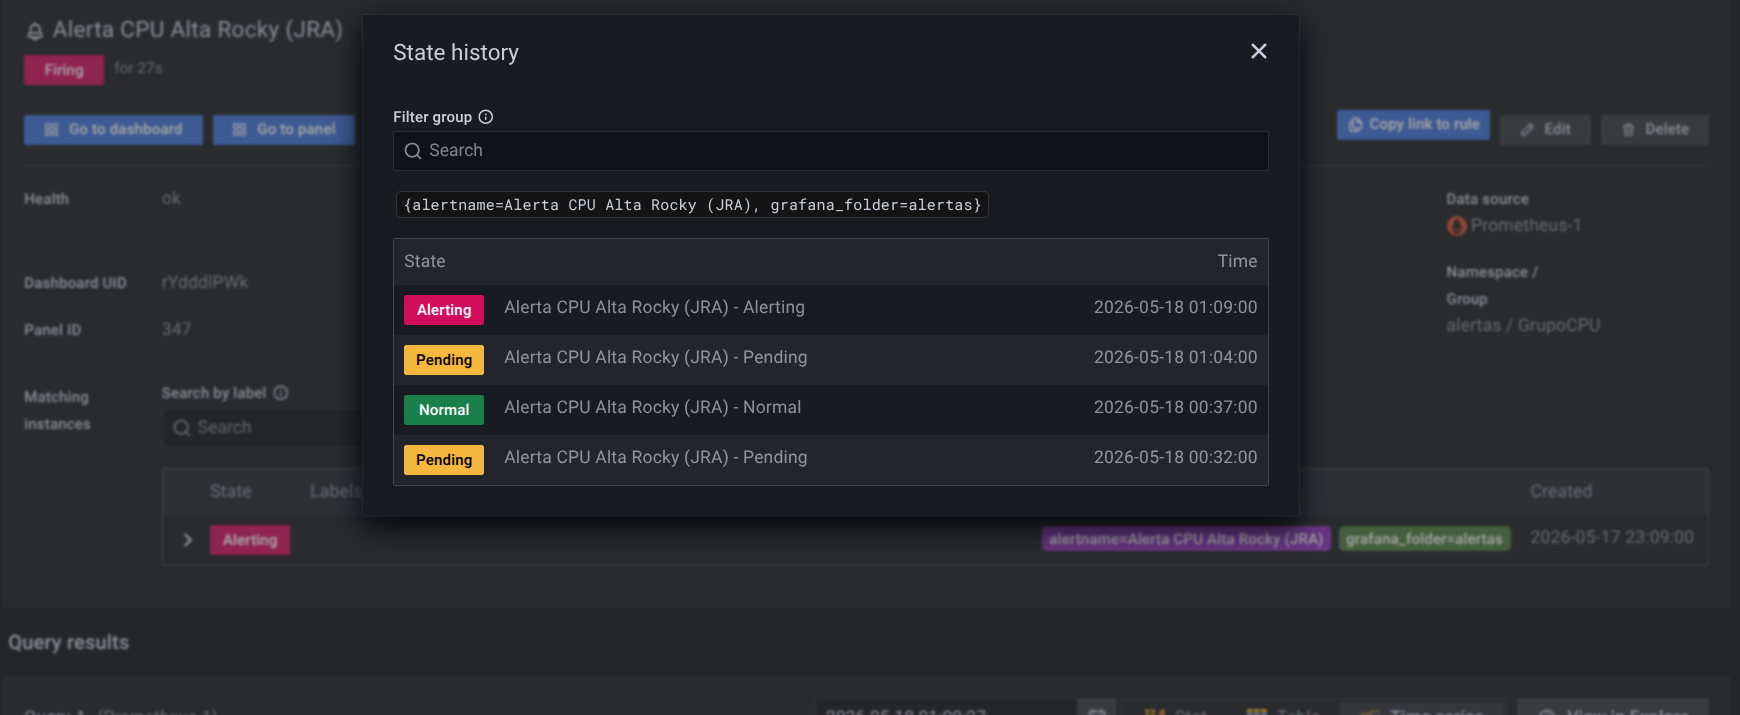
\includegraphics[width=1\textwidth]{../../capturas4/seccion4/17historial_alerta.png}

    \caption{Un vistazo al historial de la alerta.}

\end{figure}

\begin{figure}[H]
    \centering

    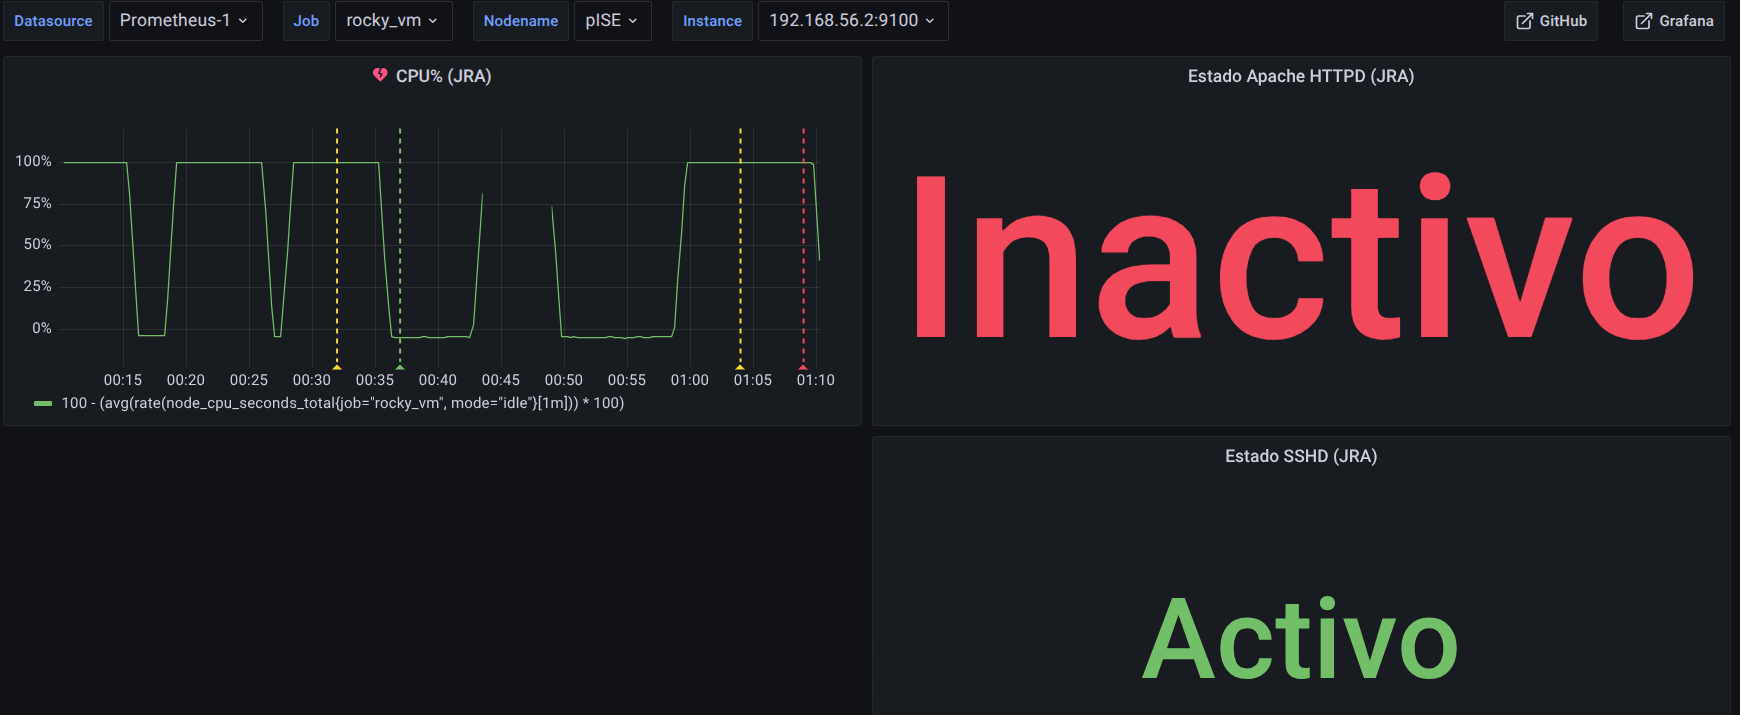
\includegraphics[width=1\textwidth]{../../capturas4/seccion4/18pos_alerta.png}

    \caption{Después de saltar la alerta y terminar stress, el consumo de CPU ha bajado.}

\end{figure}

Se pueden observar varias subidas y bajadas del consumo de CPU debido a varias pruebas realizadas para activar la alerta.



\subsection{Explicación general.}

Para completar este ejercicio, se ha usado los archivos dados por el guión para levantar docker.
\\
En una máquina virtual Rocky Linux se ha instalado Node Exporter, configurándolo como un servicio 
automático del sistema para que funcione de forma ininterrumpida en segundo plano. Aegurando antes 
que el programa tenga los permisos necesarios para ejecutarse y que el firewall permita el tráfico 
por el puerto 9100, que es el que usa el programa para enviar la información a Prometheus.
\\
Después de las configuraciones de prometheus, se paso a configurar los paneles del dashboard de Grafana. 
Se han creado dos paneles para monitorizar el puerto 80 (HTTP) y el puerto 22 (SSH), comprobando que funcionaran 
al apagar apache y que mostrara los datos correspondientes.
\\
Por ultimo se creó una alerta para el consumo de CPU, con un umbral del 75\%, y se ha ejecutado el comando stress 
para simular una carga de trabajo que dispare la alerta. Se realizó varias veces de ahí que en la captura de la gráfica 
y en el historial se puedan observar varias subidas y bajadas del consumo de CPU, fueron errores de poco tiempo del 
programa stress y de malas configuraciones del tiempo que la alerta tomaba como media de tiempo para el calculo del
uso de CPU. Una vez solucionados estos errores, se pudo activar la alerta correctamente y observar su funcionamiento.


\end{document}